\documentclass{article}
\usepackage{graphicx}
\author{John Hammond}
\title{TE 401 Final Presentation FA19}

\begin{document}

%title followed by blank space before next pager
\maketitle
\tableofcontents
\newpage

%introduction and background on the project
\section{Motivation for the Augmented Listening Project}
Augmented listening and the work we are doing here will change the way we hear and perceive\
the world around us. The idea of augmented listening is to utilize microphone arrays of any size to alter the way we hear audio.\
Effects such as source separation, dynamic range compression, and selective attenuation are all examples of digital signal\
processing in the context of hearing. Devices like hearing aids are very common and help people by amplifying the sounds around\
them and performing basic dynamic range compression.  Hearing aids, however, are limited in their capabilities due to the small\
number of microphones available and the relatively small amount of processing power. They struggle in loud environments\
with multiple sources as well as reverberant environments.  Hearing aids are only one example of augmented listening\
technology, and applications go far beyond this.

We aim to create\
an open hardware platform with support for large numbers of microphones and complex signal processing algorithms.\
This hardware platform will function as a proof of concept for our own signal processing applications as well as those\
of other researchers across the world.  The basic platform is based upon a Cyclone\textsuperscript{\textregistered{}}\
V SoC system, with support for both\
hardware logic and software applications on the ARM cores. Our implementation supports I2S microphone data streams as\
inputs for processing.

%descripton of current hardware
\section{Current Hardware Platform}

\subsection{FPGA}
The FPGA is programmed to receive I2S data, store samples in DDR3 memory buffers, and to support real-time\
signal processing cores.  We will mostly describe the hardware as it relates to recording.

\subsubsection{I2S}
Our array prototypes have all consisted of MEMS mcirophones, which send their bitstream over the I2S bus.\
We chose these microphones because they are very cheap and easy to prototype with. Two microphones share a sample\
clock, right/left select clock, power, and a data line. The right and left channel alternate sending thier 16\
bit samples. These samples are then pieced together at the I2S master into a coherent right and left data\
stream. These master cores are implemented in the FPGA fabric. Refer to figure \ref{i2s_timing} for an example of\
a typical I2S data transfer.

\begin{figure}[h]
	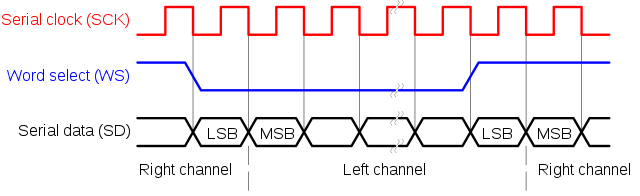
\includegraphics[scale=.5]{i2s_timing.png}
	\centering
	\caption{I2S timing diagram (wikipedia citation needed)}
	\label{i2s_timing}
\end{figure}

\newpage

\subsubsection{DMA Controller and Buffers}
Recording audio from a large number of microphones is a challenge and is one of the features of our\
open platform. There is 7.68 Mbit of space allocated in memory for the samples from each of the 10\
microphones. Each of the five I2S masters hold the lastest valid 16-bit sample for each microphone\
on its output register. 


\end{document}